\documentclass{standalone}
\usepackage[usenames,dvipsnames]{xcolor}
\usepackage{tikz}
\usetikzlibrary{decorations.pathreplacing}

\begin{document}

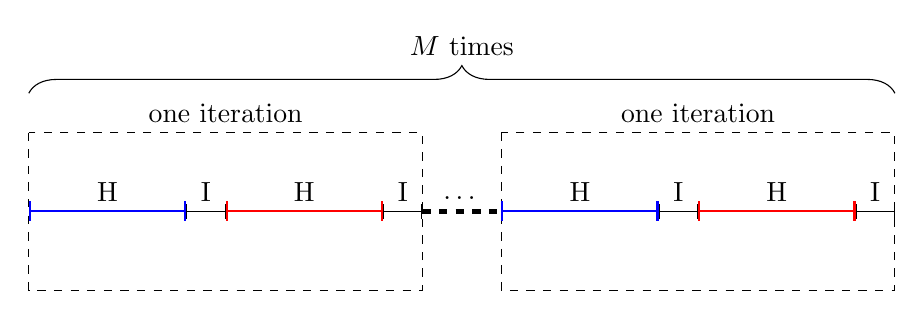
\begin{tikzpicture}[xscale=0.5, yscale=.5]

%% Define a box
% TO REMOVE
%\node (X) at (-2, -5) {};
%\node (Y) at (40, 5) {};
%\draw (X) rectangle (Y);

%% Define the nodes
% b = begin (segment)
% e = end (segment)
% tl = top left (rect)
% br = bottom right (rect)

\coordinate (Ab) at (0, 0);
\coordinate (Ae) at (2, 0);

\coordinate (IT1tl) at (2, 2);
	\node [above] at (7, 2)  {one iteration};
	\coordinate (H11b) at (Ae);
	\coordinate (H11e) at (6, 0);
	\coordinate (I11b) at (H11e);
	\coordinate (I11e) at (7, 0);
	\coordinate (H12b) at (I11e);
	\coordinate (H12e) at (11, 0);
	\coordinate (I12b) at (H12e);
	\coordinate (I12e) at (12, 0);
\coordinate (IT1br) at (12, -2);

\coordinate (DOTb) at (I12e);
\coordinate (DOTe) at (14, 0);

\coordinate (ITMtl) at (14, 2);
    \node [above] at (19, 2)  {one iteration};
    \coordinate (HM1b) at (DOTe);
    \coordinate (HM1e) at (18, 0);
    \coordinate (IM1b) at (HM1e);
    \coordinate (IM1e) at (19, 0);
    \coordinate (HM2b) at (IM1e);
    \coordinate (HM2e) at (23, 0);
    \coordinate (IM2b) at (HM2e);
    \coordinate (IM2e) at (24, 0);
\coordinate (ITMbr) at (24, -2);

\coordinate (Gb) at (24, 0);
\coordinate (Ge) at (27, 0);

%% Draw the times sequences
%\draw [|-|, thick, ForestGreen] (Ab) to node [above, black] { A }  (Ae);

\draw [dashed] (IT1tl) rectangle (IT1br);
\draw [|-|, thick, blue] (H11b) to node [above, black] { H } (H11e);
\draw [|-|] (I11b) to node [above] { I } (I11e);
\draw [|-|, thick, red] (H12b) to node [above, black] { H } (H12e);
\draw [|-|] (I12b) to node [above] { I } (I12e);

\draw [ultra thick, dashed] (DOTb) to node [above] { \dots } (DOTe);

\draw [dashed] (ITMtl) rectangle (ITMbr);
\draw [|-|, thick, blue] (HM1b) to node [above, black] { H } (HM1e);
\draw [|-|] (IM1b) to node [above] { I } (IM1e);
\draw [|-|, thick, red] (HM2b) to node [above, black] { H } (HM2e);
\draw [|-|] (IM2b) to node [above] { I } (IM2e);

%\draw [|-|, thick, ForestGreen] (Gb) to node [above, black] { G } (Ge);

\draw [decorate, decoration={brace, amplitude=10}] (2, 3) to node [above=10pt] { $M$ times } (24, 3);

\end{tikzpicture}


\end{document}
